\PassOptionsToPackage{svgnames,x11names}{xcolor}

\documentclass[tikz,margin=0pt]{standalone}

\usepackage{tikz,tikz-3dplot}
\usepackage{pgfplots}
\usepackage{tkz-euclide}



\begin{document}
    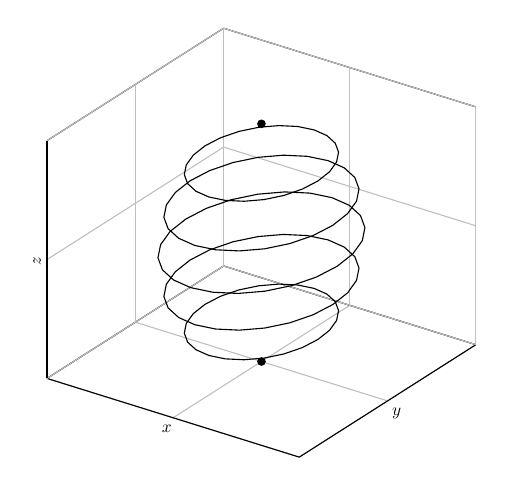
\begin{tikzpicture}[every node/.style={scale=.625}]
        \begin{axis}[
            width = 200pt,
            height = 200pt,
            grid = major,
            view={35}{30},
            xmin = -5, xmax = 5,
            ymin = -5, ymax = 5,
            zmin = -5, zmax = 5,
            xlabel = {$x$},
            ylabel = {$y$},
            zlabel = {$z$},
            ticks = none,
            ]
            \foreach\h in {-10/3,-5/3,0,5/3,10/3}
            {
                \pgfmathparse{sqrt(1-(\h)^2/5^2)}
                \let\s\pgfmathresult
                \addplot3[domain=0:360,samples y=0]({3*\s*sin(x)},{4*\s*cos(x)},{\h});
            }
            \node[fill, shape=circle, fill, minimum size=5pt, inner sep=0pt] at (0,0,5) {};
            \node[fill, shape=circle, fill, minimum size=5pt, inner sep=0pt] at (0,0,-5) {};
        \end{axis}
    \end{tikzpicture}
\end{document}